\chapter{Présentation du projet}


\section{Contexte}
\begin{paracol}{2}%
  Dans le cadre du projet DSCATT, nous, Paul Chapron (IGN), Romain Reuillon (CNRS) et Etienne Delay (CIRAD) avons animé une semaine d'atelier à Diohine sur le territoire de l'observatoire IRD de Niakhar(fig. \ref{fig:photoAtelier}). Ils s'inscrivent dans différentes réflexions de recherche autour de l'exploration\\
  d'accompagnement, et les théories de la viabilité appliquées aux systèmes multi-agents.
  Ces journées d'atelier ont mobilisé quatre acteurs locaux sur cinq jours:
  \begin{itemize}
    \item Paul Sene +221 77 623 60 93
    \item Marcel Latyr Diouf +221 77 198 41 06
    \item Marie Hélène Ndjira +221 77 072 54 60
    \item Idrissa Faye +221 77 408 24 76
    \item Robert Diatte +221 77 426 60 82
  \end{itemize}

\switchcolumn %Sérères
  No kaa farna no projet DSCATT, In Paul Chaperon (IGN), Romain Reuillon (CNRS), fa Etienne Delay (CIRAD) I ndjiala semene moum diohine saax na paan ale IRD djialaa, caalel ke refaa kaa farna na saak, fo a kalat no kaa farna no mbi ir ne na djiega, no niaal betik, i djiala ten fo wiin naxuk

  \begin{itemize}
    \item Paul Sene 77 623 60 93
    \item Marcel Latyr Diouf 77 198 41 06
    \item Marie Hélène Ndjira 77 072 54 60
    \item Idrissa Faye 77 408 24 76
    \item Robert Diatte 77 426 60 82
  \end{itemize}
\end{paracol}

  \begin{figure}
    \begin{center}
      \includegraphics[width=8cm]{img/atelier_niakhar.jpg}
    \end{center}
      %légende de l'image
    \caption{Atelier dans la case de Réunion à Niakar. Sur la photo, sont présent, Romain Reuillon, Paul Chapron, Paul Séné et Marcel Latyr Diouf}
    \label{fig:photoAtelier}
  \end{figure}

\begin{paracol}{2}

  L'enjeu de cette semaine d'atelier était de formaliser avec les acteurs leur représentation du système d'interaction et de solidarité dans lequel s'inscrit la gestion collective de l'espace à travers la survivance des jachères communautaires. Le système de jachère est lui-même considéré comme un élément clef des processus de maintien de la fertilité des sols et donc un proxy sur les questions de stockage de carbone dans les sols.

  \switchcolumn %Sérères

  Kaam semene nene i djial na ten redu i det lokoor ne djieg na no ka far na na niadjinodale na kop ale diohine, fo ne a toss ake a mbi tel, yam a toss a kene kaa fog no ke modj na o xaad na lang ke
  Kam semene nene, we mbog na no calel ke a ndjiaba no gua o ferand ole I nga na na niadjinod a lene

\end{paracol}

  À l'issue de la semaine, les participants ont pu valider une première version de leur système qu'on retrouve ici : \url{https://github.com/ElCep/DSCATT/tree/master/PARDi}

  Ce document a été rédigé en s'appuyant sur des notes prises sur le terrain :
  \begin{itemize}
    \item Note de Paul : \url{https://hackmd.openmole.org/Rck70wm6Qmu_ztM0M03--w?view}
    \item Note d'Etienne : \url{https://hackmd.openmole.org/qhPAjsJGRbiOQYIItbwPww#}
  \end{itemize}



\section{PARDi, un outil de mise en lumière de l'agencement des éléments du système.}

\subsection{Le diagramme comme outil de représentation du système}

\begin{paracol}{2}
  La méthode PARDI est une évolution des spécifications de ARDI\cite{etienne_ardi_2011} qui relève de la capacité de l'outil à expliciter des implicites et rendre visible des hypothèses de modélisation. Cette méthode mobilise des diagrammes pour représenter à la fois les éléments constitutifs du système et les interactions entre ces éléments.

  Ces diagrammes sont constitués de nœuds représentés par des cercles ou des ellipses, et d'arcs, représentés par des flèches, qui relient les nœuds.

  \switchcolumn %Sérères

  Ke I ngoyaa PARDI a refa a niadjnod ala andona yee ka I ngot mandarga kaa andona yee xan da modji o lerand a in a kalat ake I teg na, mandarga kene ka ngotel nen cialir no kaa farna no lokor ne.

  Mandarga kene kaa nandit ne na kimb a dak a ka nandit na nen a pano fo nen a xali.

  \switchcolumn %Français

  Dans un diagramme PARDI comme ceux que nous allons inclure dans la suite de ce rapport, les nœuds représentent des acteurs ou des ressources, et les arcs représentent des interactions entre ces acteurs, entre ces ressources ou entre ces acteurs et ces ressources.

  \switchcolumn %Sérères

  No ke I ngoyaa PARDI mene koy a pano ke na ndef ka we na mbi a, fo o ndjirnio nge, so a xali le ref ke lokoor na den

\end{paracol}

%inclusion d'une mage dans le document
\begin{figure}[h!]
  \begin{center}
    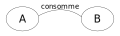
\includegraphics[width=8cm]{img/diagramme_simple.png}
  \end{center}
    %légende de l'image
  \caption{Exemple d'un diagramme simple, ou un acteur A est relié à une ressource B par une interaction.}
  \label{simple_interac}
\end{figure}

  Comme les nœuds et les arcs sont nommés, il devient facile de faire une phrase qui décrit l'interaction de façon concise. Par exemple avec la figure \ref{simple_interac}, on pourrait former la phrase suivante : « A consomme B». Plusieurs arcs peuvent exister entre deux mêmes nœuds pour représenter des interactions différentes.\todo{Je pense que ce paragaphe n'est pas traduit}

\section{Modélisation PARDI du système de Diohine}

\subsection{Les Acteurs}

\begin{paracol}{2}
  Par la suite nous utiliserons les termes suivants:
  \begin{itemize}
    \item \textbf{Acteur/role}: personne physique partie prenante dans le système étudié
    \item \textbf{Participant} : personnes physiques concourant à la co-construction du modèle durant l'atelier. C'est donc un sous-ensemble des "acteurs".
  \end{itemize}

  \switchcolumn %Sérères

  Xa ta djieg kaa i mbug ko ngoyaa :
  \begin{itemize}
    \item \textbf{We na mbi a}: wiin wa na mbug ko mbi a no ke I sakaa
    \item \textbf{Lalay we}: win wa I mbug lamtira no ka farna na sakale I sakaa
  \end{itemize}



\vspace{0.5cm}
  \switchcolumn %Francais
  La méthode PARDI propose d'interroger des participants évoluant dans un même système. Ils participent à co-construire d'un diagramme d'interactions entre acteurs sur la base de la connaissance qu'ils ont de ce système. La méthode a pour effet de les faire réfléchir sur la réalité du système dans lequel ils évoluent. Les échanges de points de vue stimulent leur créativité en mettant en lumière des liens entre certains objets de leurs quotidiens. L'enjeu du travail de modélisation conceptuel avec PARDI est d'accompagner par un mode de représentation schématique la réflexion sur le fonctionnement du système \cite{becu_les_2010}.\\

  \switchcolumn %Sérères

  PARDI kaa bug ko lamtaa wiin we na yo nuwa na niadjinodale na kop ale, ten taxu bo xan da bog fa in ne I ndjialit ka mandargal ne I mbug na nder we na mbi a fo we na layaa, ten na tax ka boo I ngalat nor a den ne tige niadj taa no ndigil, ndioktoor ne na djieg kaa kam in na tax kaa boo tige xool na in.

  \switchcolumn %Francais

  En avant propos, il nous semble important de définir le concept de cuisine, qui est un élément central de l'organisation du social du système. Une \textbf{cuisine} regroupe les personnes qui mangent ensemble et donc qui participent à l’alimentation par leur travail. Du fait de l’imbrication des systèmes de solidarité (et du lien avec la lignée maternelle).

  \switchcolumn %Sérères

  Ten taxu a djega solo lol in lay ke na xoyeel ngaak ta ref wiin wa bog na cialel too a mboga o roon

  \switchcolumn %Francais

  Le territoire fait face à un phénomène d’éclatement des cuisines.  Pour nos participants, si les femmes participent très fortement à cet éclatement, l'éducation des enfants y joue aussi un rôle important, quand les sanctions d'autres membres de la famille sont mal vécues par les parents. Cela produit un phénomène : «Avec l’éclatement des cuisines, il y a de moins en moins de place pour les fainéants. Tout le monde doit travailler à fond.»

  \switchcolumn %Sérères
  I nga a yee kaak mayu kaa ngadjiwataa, too sax no we I lamtoora I anda yee mayu ten no rew we xataa, fa yar fe no xa ciadj axe yoo a foga ten yaa ta referna ling, kam a kadjiale no kak ken a taxa bo fop a ndjiala, ten taxu boo ke I ngoya we na mbi a a ref ka

  \switchcolumn %Français
  Les acteurs représentés dans le modèle sont:
  \begin{itemize}
    \item \textbf{Agriculteur}: paysan travaillant la terre, soucieux de sa productivité, produisant de l'arachide, du mil, des cultures de rente et des plantes fourragères. Il accueille et nourrit le bétail des pasteurs transhumants, qui vont fertiliser son champ en retour. Il supporte les frais d'abreuvage et de soins aux bêtes des transhumants.
    \item \textbf{Pasteur}: éleveur utilisant pour nourrir son bétail les herbes fourragères, les résidus de récolte (tiges de mil, fane d'arachide, etc), ou le pâturage dans les jachères ou les couloirs entre les cultures. Il contribue par son cheptel à la fertilité des sols. Il accompagne étroitement le paysan dans la fertilisation de son sol.
    \item \textbf{Eleveur/Transhumant}: pasteur (nomade) s'arrêtant quelques semaines dans le village pour faire pâturer son bétail sur les jachères et les pâturages "couloirs" entrer les cultures. Il participe en retour à la fertilité des champs ponctuellement.
    \item \textbf{Chef de cuisine} (ou chef de famille ou chef de ménage): homme ayant la responsabilité de nourrir, éduquer, soigner, soutenir (financièrement), et incarner la représentation morale de tout ou partie de la famille. C'est souvent le plus âgé de la famille. Il supervise et participe (s'il le peut toujours) aux travaux de la cuisine.
    \item \textbf{Chef de concession} (ou chef de maison): homme ayant la charge d'entretenir et de partager la paix sociale au sein des différentes cuisines qui la compose. Il a un rôle de conseil envers ses chefs de cuisine.
    \item \textbf{Notable} ("personne qui a la parole" litteralement en Serer): personne morale importante dans le village, soucieuse du bien être social de la communauté. Il est écouté dans le village (ex: instituteur, médecin, imam, saltigué, marabout, etc).
    \item \textbf{Vieille maman}:  femme âgée, sage, capable de guider les membres de la communauté. Elle n'est plus comptée dans les activités de la famille. Elle a une autorité coutumière envers les autres femmes.
    \item \textbf{Chef de village}: autorité coutumière du lieu de peuplement, reconnue par l'autorité centrale de l'état. Il est élu à vie (sauf destitution en cas de malhonnêteté avérée) par les chefs de cuisine sous l'égide de l'autorité centrale (via les sous-préfets). Il est l'intermédiaire entre l'autorité centrale et les habitants. Il intervient dans les activités courantes du village (paix sociale, éducation, distribution des engrais, etc).
    \item \textbf{Conseil municipal}: ensemble d'individus qui sont élus aux élections locales et qui s'insèrent dans le droit positif et les institutions de l'état. Il traite de nombreux aspects de la vie de la population, entre autres il prend en charge les conflits sur les territoires et mobilise les lois de l'état pour les résoudre  (commission domaniale).
    \item \textbf{Sous-préfet}: Représentant de l'état décentralisé sur les territoires. Il prend en charge les conflits quand le droit traditionnel n'a pas réussi à trouver une solution convenable pour les différentes parties intéressées. Il contrôle la légalité des activités du conseil municipal.
    \item \textbf{Saltigué}: voyant et devin qui officie lors de la cérémonie divinatoire de la première chasse. Ses prédictions portent sur la météo, les catastrophes et les remèdes pour y faire face. Il a également un rôle de soignant. Un saltigué a un ou plusieurs quartiers sous sa juridiction.
    \item \textbf{Banque de Céréales}: Structure locale (à l'échelle d'un quartier) qui prête des céréales aux agro-pasteurs contre un remboursement ultérieur et vend des céréales. Chaque cuisine est libre de contribuer au stock de la banque en donnant une portion de sa récolte.
  \end{itemize}

  \switchcolumn %Sérères
  \begin{itemize}
    \item \textbf{Xoxox We}: o kiin oxa na djirniu waa no lang ke to a xalataa ke ta xotit kaa ten. Ten ref o xe na xoxaa kaaf fo a arer fo ka ta niow nit na cieguelum, a refa it o xaa na dal na we na molaa ndax da ndoss a nin xaa kolum, a na dimle ta na yer na le no mumen ke fo na badnale.
    \item \textbf{O KAYNAAK OXE}: oxe na yaaraa mumen to a niownitaa dat, fo fo goonia arer fo ngangaf, a gay taa na xa kur axe fo a toss ake, ten it a foga no we na ndosaa xa kol axe
    \item \textbf{O MOLAAN OXE}: ten ref o xe na molaa nder saate fa saate a gay taa no xa kur axe fo na toss ake, tenoo ka dossaa lang ke
    \item \textbf{O YAAL NGAAK}: o kiin oxe na niownaa basil ne to a saytuxaa o wod ole fo fa yar fe to a dam taa mbasil ne no cioxla lakass ke, ten ref oxe yob na ref o mak no ngak ne
    \item \textbf{O YAAL MBIND}: o kiin oxe na saytuwaa diam fe ref nan der kaak ke ndef na no mbin ne, ka niaxaa o yaal kaak ke no paax
    \item \textbf{WE NDJIEG NA ONIUXUR NO SAATE}: kiin o djiegu sagu so sax: nan nen a eliman, saltiki, o metar, o sir no xe
    \item \textbf{YAAY MAAK KE}: a nogoy a ke ndjiega ter na cialel, to a saytuwaa djiam no sax le, fo no xa cieg axe no sax le
    \item \textbf{O YAAL SAATE}: o kiin oxe sax la a ndod na a yon ten fa superefe yam o woor um fo diof um, ten refanu a superefe no sax le, a na saytuxaa it djiam fe fo fa yar fe, fo ku warena o xaadjir nan ne na angare no saaax le
    \item \textbf{O YAAL SAATE}: o kiin oxe sax la a ndod na a yon ten fa superefe yam o woor um fo diof um, ten refanu a superefe no sax le, a na saytuxaa it djiam fe fo fa yar fe, fo ku warena o xaadjir nan ne na angare no saaax le
    \item \textbf{KOSEYE}: wiin waa ndodena no woote, so a saytuwaa a dat ale no mad oxe, nden na ngate a yaa ndawir a djiegna no lang ke
    \item \textbf{SUPERE FE}: o kiin oxe mofan na men mat ne, ten na xate a tawir ke yaa ta waagandena o fi it no saas laa, a naa fodranda a sax ake
    \item \textbf{SATIKI}: o kaaga oxaa na layaa ke ta ga na yaa o miss a fad na, a na layaa yiit na teb ake fo no ku waag na o yak ndig, a refa yiit o dadax no saax
    \item \textbf{NDAP KAFF NO SAAX}: mangasin na saax a mbokataa kaaf soo a ndawniran to a ndjikwa ten
  \end{itemize}
  \switchcolumn %Francais

  Les acteurs ci-dessous ne nécessitent pas d'explicitation approfondie, leur nom étant assez explicite.

  \begin{itemize}
    \item École
    \item Revendeur de semence
    \item Revendeur d'engrais
    \item Animal de trait : âne et cheval
    \item Petit ruminant : mouton et chèvre
    \item Grand ruminant : bœuf et vache
  \end{itemize}
  \switchcolumn %Sérères
  Ngaak nu ref na a waa fog yaa ta bug na. We yok na ndjiar ke I layaa ke da ndef na yam I andaan
  \begin{itemize}
    \item Ekol ne
    \item Oxe na djikwaa ax
    \item Oxe na djikwaa angare
    \item Mumen ke na ngoox tel
    \item Mumen teb ke: mbaal, fambe
    \item Mumen maak ke: naak ke
  \end{itemize}

\end{paracol}

\subsection{L'atelier de modélisation PARDI à Diohine }

\begin{paracol}{2}
  Dans le cadre du questionnement autour du stockage de carbone dans les pratiques agricoles du projet DSCATT, nous nous \\
  sommes intéressés à la gestion communautaire de la jachère dans la commune de Diohine.

  La jachère est la pratique agricole visant à laisser au repos une parcelle entre deux cultures, généralement sur une période d'un an. À Diohine, cette jachère s'intercale la plupart du temps au sein d'un assolement triennal: Mil, Arachide, Jachère.

  Ainsi la jachère a le double avantage de maintenir une fertilité élevée et de stocker du carbone. Ainsi s'intéresser au maintien d'une jachère gérée en commun semble être un proxy du stockage de carbone tout en permettant à la population de subvenir à ses besoins alimentaires.

  \switchcolumn %Sérères

  No ka farna na laamtax no kaadel ole no lang ke, fo na kookod ale no prose le na xoyel DSCATT, a toss ake diohine a soxal a in.

  A toss o refa o niotin o kol ka fad na o xiid nder tuflax dik, no saax le diohine a toss a kene o we ndjiega tiig dik ku refna ndadkanderna a toss a djieg: kaaf, arer, a toss.

  Nene a toos ale a djieg tu xa ndjirin xa dak: xaadin lang ke so a niowdatin.

  \switchcolumn %Francais
  L'atelier de modélisation réunit:
  \begin{itemize}
    \item deux agro-pasteurs
    \item un agriculteur
    \item une agri-pastrice vieille maman
  \end{itemize}

  \switchcolumn %Sérères

  Keene taxu boo djieg a toss a kaa saax fop mbog na a waa tax lang ngad to saax le ndjiega ten niowir. Mbokatax ne tax na I liba kaa fokat
  \begin{itemize}
    \item Dik waa na ngoxaa ta ngayaa
    \item O koxox
    \item O tew oxa na xooxaa ta gayaa
  \end{itemize}

  \switchcolumn %Francais

  Ils participent à co-construire le diagramme d'interaction d'un système agro-pastoral à l'échelle de la ville de Diohine, tentant de répondre à la problématique que nous pouvons formuler de la manière suivante : «Comment se maintient la jachère communautaire de Diohine ?»

  Cette question fait suite à une première consultation à Diohine en mai 2021 lors de laquelle une inquiétude doublée d'une aspiration très forte a été formulée (voir figure \ref{aspiration}) : Comment préserver la jachère communautaire à Diohine ?\cite{perrotton_definition_2021}

  \switchcolumn %Sérères

  Den na tax kaa i mbago ndjial madargal ne na ref ka lokoor ne djieg na kam den no saax le diohine, to ten na tax kaa I mbaago tontoox a laamtax ale refna nam I mbi kaa mboo a toss ake mbatke diohine.

  La amtax nene a taxa boo na 2021, a fi a a in o ndjiaxdatan no kaa farna no bug bug ke diohine, nam I mbi kaa boo a toss ake mbat ke

\end{paracol}

\begin{figure}[h!]
  \begin{center}
  %taille de l'image en largeur remplacer "width" par "height" pour régler la hauteur
  \includegraphics[width=15cm]{img/aspiration_formulee.jpg}
  \end{center}
  %légende de l'image
  \caption{Diagramme des aspirations proposées par un groupe stratégique lors des ateliers d'avril 2021.}
  \label{aspiration}
\end{figure}

\begin{paracol}{2}
  Or, pour entrevoir comment préserver cette jachère communautaire à l'avenir, nous devons d'abord nous intéresser à ce qui fonde son existence; et c'est à cette question que nous allons nous intéresser dans les pages suivantes.

  Aussi pouvons-nous reformuler cette question en termes plus académiques et généraux de la façon suivante : \textbf{Comment préserver une gestion foncière concertée de la fertilité ?}

  Le travail de modélisation a amené les participants à définir une centaine de nœuds et leurs arcs. Le diagramme complet est visible sur la figure \ref{diagComplet}

  \switchcolumn %Sérères

  Ndikii ke na tax kaa boo a toss ake mbat ke, ke tax na ta fiel xan ta soxal ong.

  Ten taxu o xan I supit laamtax ne yaa I lay na e nam I mbagu saytoxit lang ke mbo nguek ko kaadel ole.

  Kene a taxa mbo wiin we ndjial na fa in a bisid kaa fadna pano teemed fo a kali den.

  Mandargal nene a lal te na \ref{diagComplet}.



  \switchcolumn %Francais
  Nous avons choisi de le restituer dans ce rapport avec quatre points de vue différents :
  \begin{enumerate}
    \item les activités liées aux rôles d'agro-pasteur
    \item les mécanismes de résolution de conflit
    \item les interactions liées à la gestion collective de l'espace
    \item les réseaux de solidarités
  \end{enumerate}

  \switchcolumn %Sérères

  Kene taxu I ndjialtin no xa pasong xa naxak
  \begin{enumerate}
    \item cialel ke lokoor na fo ke o xe na xoxaa ta gayaa fia
    \item ke warena o fi boo nanoor a djieg
    \item lokoor ne wag na dieg boo fop a ndjirnoor a kop ale
    \item ke wag na tax fop a mbiyaa ling
  \end{enumerate}

\end{paracol}



\begin{figure}
  \begin{center}
  %taille de l'image en largeur remplacer "width" par "height" pour régler la hauteur
  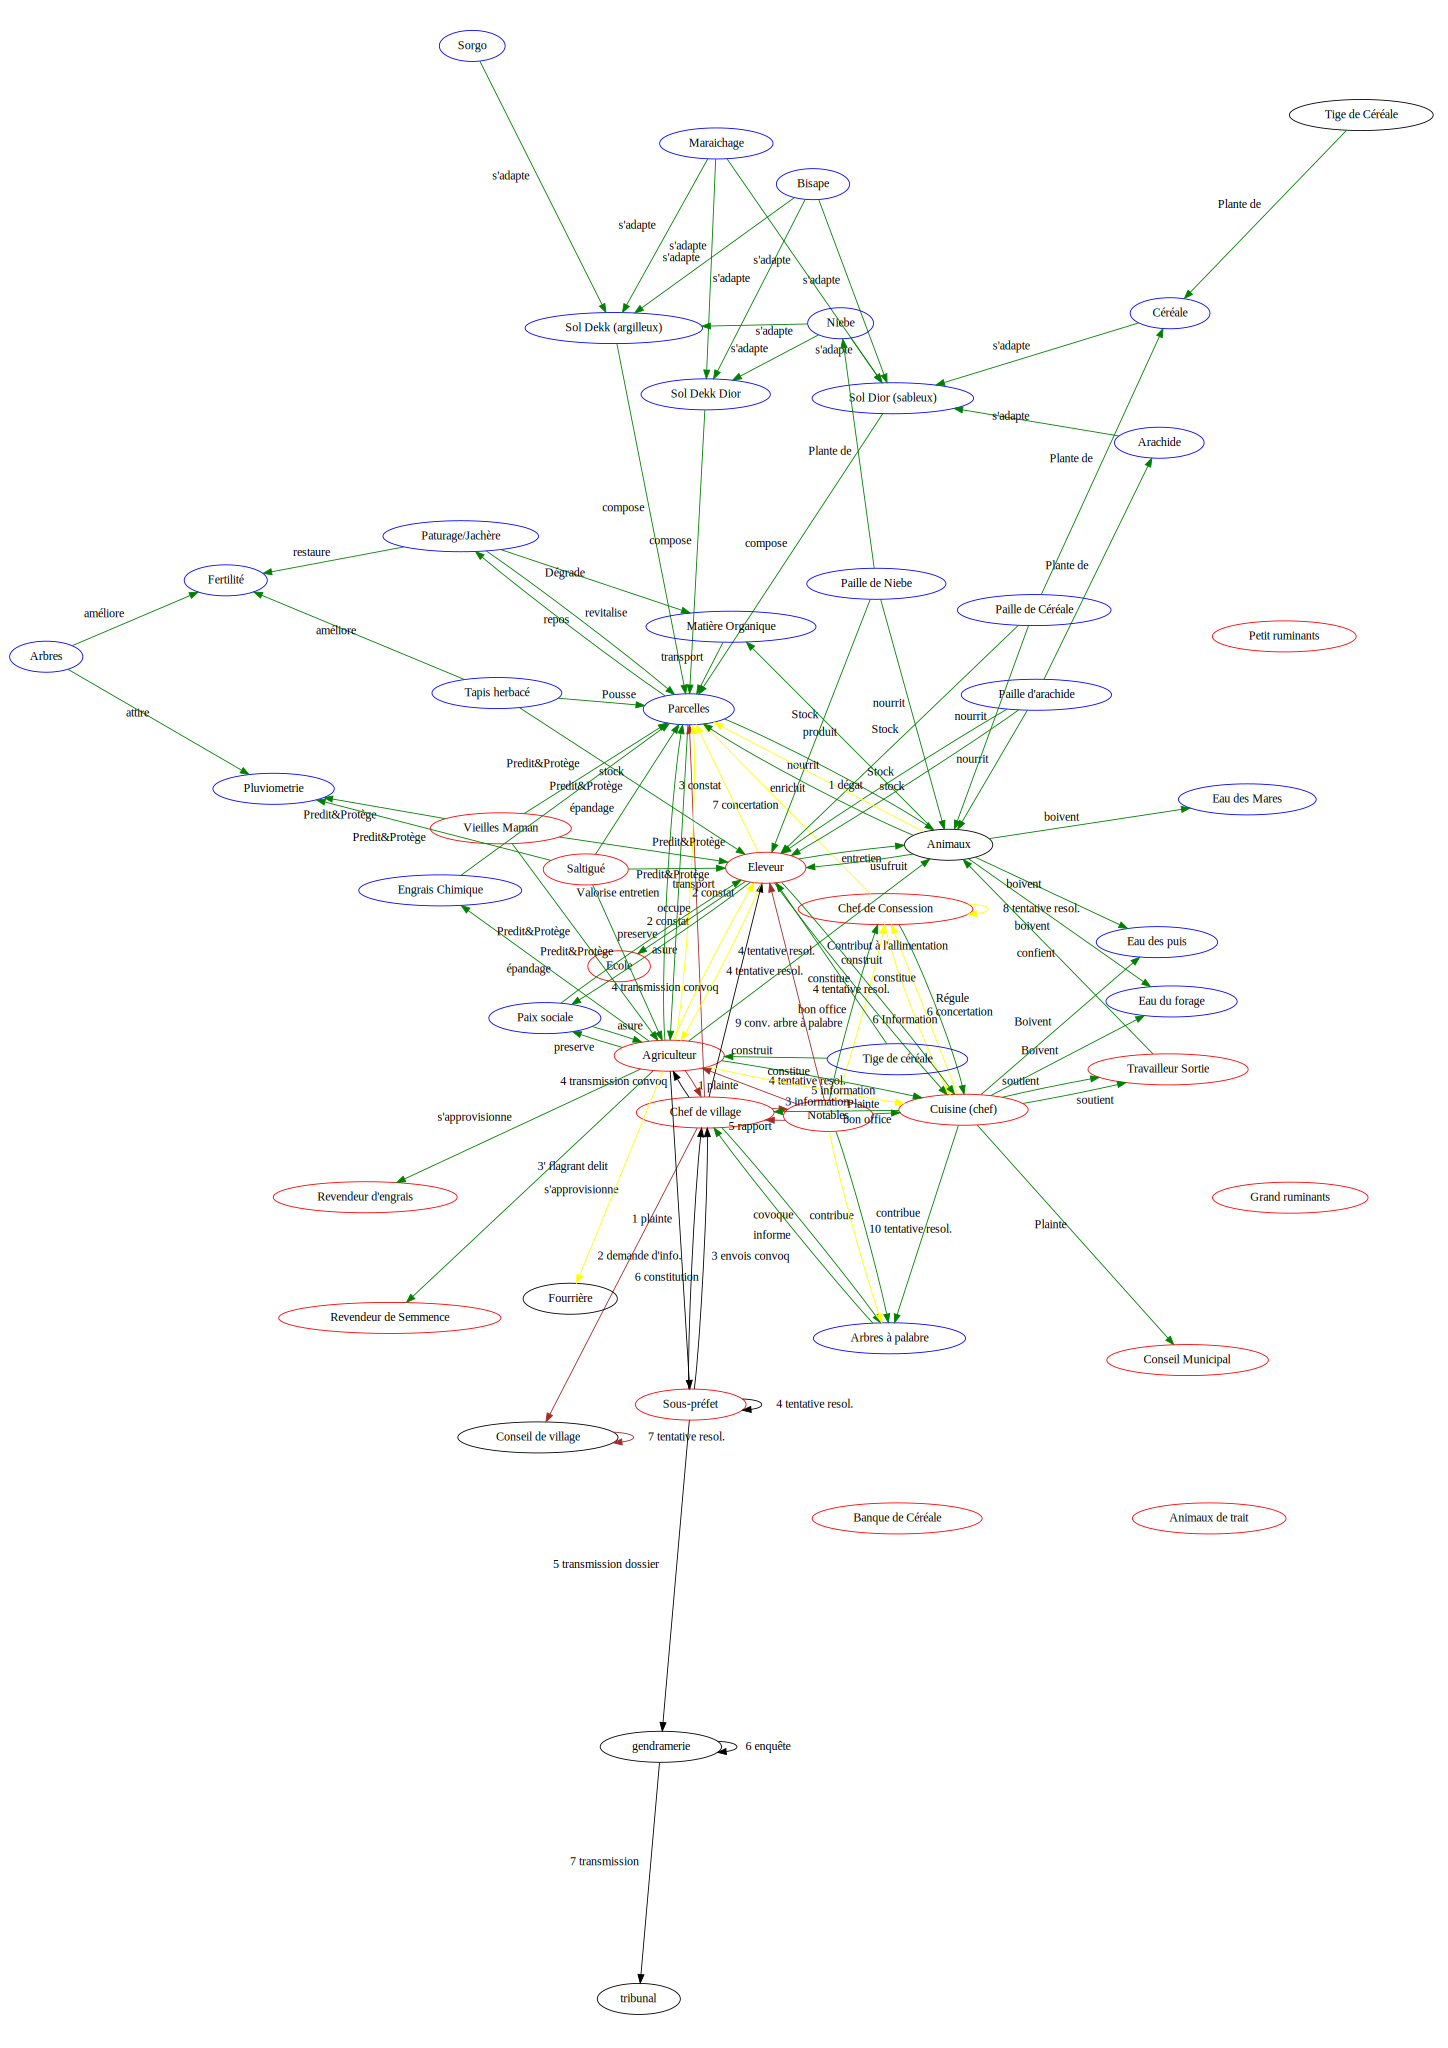
\includegraphics[width=15cm]{img/pardi_fdp.png}
  \end{center}
  %légende de l'image
  \caption{Diagramme complet des interactions relevées pendant l'atelier à Diohine }
  \label{diagComplet}
\end{figure}
